%%%%%%%%%%%%%%%%%%%%%%%%%%%%%%%%%%%%%%%%
% iz predloge:
%
% datoteka diploma-vzorec.tex
%
% vzorčna datoteka za pisanje diplomskega dela v formatu LaTeX
% na UL Fakulteti za računalništvo in informatiko
%
% vkup spravil Gašper Fijavž, december 2010
% množica popravkov v januarju, februarju marcu 2011
% verzija 29. marec 2011

\documentclass[a4paper, 12pt, ]{book} 
%openany?

\usepackage[utf8x]{inputenc}   % omogoča uporabo slovenskih črk kodiranih v formatu UTF-8 
\usepackage[slovene,english]{babel}    % naloži, med drugim, slovenske delilne vzorce
\usepackage[pdftex]{graphicx}  % omogoča vlaganje slik različnih formatov 
\usepackage{fancyhdr}          % poskrbi, na primer, za glave strani
\usepackage{amssymb}           % dodatni simboli
\usepackage{amsmath}           % eqref, npr.

\usepackage{color}		% barve

\usepackage{hyphenat}
\usepackage{hyperref}	% povezave
\hypersetup{
    colorlinks=false, 		%set true if you want colored links
    linktoc=all,    			 %set to all if you want both sections and subsections linked
    colorlinks,
    citecolor=black,
    filecolor=black,
    linkcolor=black,
    urlcolor=black
}
\usepackage[hmarginratio=3:2]{geometry}	% obrne razmerja marginov
\usepackage[nottoc]{tocbibind}	% prepreči številko za literaturo v kazalu
\usepackage{amssymb}		% oznake za množice števil, npr. N za naravna števila

%---------------------------------------------
% pseudokoda
\usepackage[chapter]{algorithm}
\usepackage[noend]{algpseudocode}
%\usepackage{algorithmicx}
\usepackage{setspace}
\newcommand{\alglinestretch}{1}
\floatname{algorithm}{Algoritem}
\renewcommand{\algorithmicrequire}{\textbf{Vhod:}}
\renewcommand{\algorithmicensure}{\textbf{Izhod:}}
%---------------------------------------------




\renewcommand{\baselinestretch}{1.3} % ustrezen razmik med vrsticami

%oznake strani
\renewcommand{\chaptermark}[1]{\markboth{\MakeUppercase{\thechapter.\ #1}}{}}
\renewcommand{\sectionmark}[1]{\markright{\MakeUppercase{\thesection.\ #1}}}
\renewcommand{\headrulewidth}{0.5pt}
\renewcommand{\footrulewidth}{0pt} 
\fancyhf{}
\fancyhead[LE,RO]{\sl \thepage}
\fancyhead[LO]{\sl \rightmark}
\fancyhead[RE]{\sl \leftmark}


\newcommand{\BibTeX}{{\sc Bib}\TeX}

\newcommand{\autfont}{\Large}
\newcommand{\titfont}{\LARGE\bf}

\setcounter{tocdepth}{1}	      % globina kazala

% konstrukti
\newtheorem{izrek}{Izrek}[chapter]
%\newtheorem{trditev}{Trditev}[izrek]
\newenvironment{dokaz}{\emph{Dokaz.}\ }{\hspace{\fill}{$\Box$}}

% todo tag
\newcommand{\TODO}[1]{\textcolor{red}{#1}}

\newcommand{\clearemptydoublepage}{\newpage{\pagestyle{empty}\cleardoublepage}}


% Referenciranje algoritma
\newcommand{\refalg}[1]{(Alg. \ref{#1})}





\begin{document}
\selectlanguage{slovene}
\frontmatter
\setcounter{page}{1} %
\renewcommand{\thepage}{}       % preprecimo težave s številkami strani v kazalu 



	%---------------------------------------------
	%naslovnica
	 \thispagestyle{empty}%
	   \begin{center}
	    {\large\sc Univerza v Ljubljani\\%
	      Fakulteta za računalništvo in informatiko}%
	    \vskip 10em%
	    {\autfont Nejc Ramovš\par}%
	    {\titfont Problem izomorfnega podgrafa \par}%
	    {\vskip 2em \textsc{DIPLOMSKO DELO\\NA UNIVERZITETNEM ŠTUDIJU}\par}%
	    \vfill\null%
	    {\large \textsc{Mentor}: prof.~dr.~Borut Robič\par}%
	    {\vskip 2em \large Ljubljana, 2013 \par}%
	\end{center}
	
	% prazna stran
	\clearemptydoublepage




	%---------------------------------------------
	%copyright stran
	\thispagestyle{empty}
	\vspace*{8cm}
	{\small \noindent
	Rezultati diplomskega dela so intelektualna lastnina Fakultete za ra\-ču\-nal\-niš\-tvo in informatiko Univerze v Ljubljani. 
	Za objavljanje ali izkoriščanje rezultatov di\-plom\-ske\-ga dela je potrebno pisno soglasje Fakultete za ra\-ču\-nal\-niš\-tvo in 
	informatiko ter mentorja.}
	
	% prazna stran
	\clearemptydoublepage
	



	%---------------------------------------------
	% stran 3 med uvodnimi listi
	\noindent
	Namesto te strani {\bf vstavite} original izdane teme diplomskega 
	dela s podpisom mentorja in dekana ter žigom fakultete, ki ga diplomant
	dvigne v študent\-skem referatu,  preden odda izdelek v vezavo!
	
	% prazna stran
	\clearemptydoublepage




	%---------------------------------------------
	% izjava o avtorstvu
	\vspace*{1cm}
	\begin{center} 
	{\Large \textbf{\sc Izjava o avtorstvu diplomskega dela}}
	\end{center}
	
	\vspace{1cm}
	
	\begin{tabbing}
	\hspace*{4cm}\= \kill
	Spodaj podpisani \> Nejc Ramovš,  \\[0.3cm]
	z vpisno številko \>  63070162, \\
	\end{tabbing}
	
	\noindent sem avtor  diplomskega dela z naslovom:
	 
	
	\vspace{0.5cm}
	\emph{Problem izomorfnega podgrafa}
	
	\vspace{1.5cm}
	\noindent S svojim podpisom zagotavljam, da:
	\begin{itemize}
		\item sem diplomsko delo izdelal samostojno pod mentorstvom\\ prof.~dr.~Boruta Robiča,
	
		\item	so elektronska oblika diplomskega dela, naslov (slov., angl.), povzetek (slov., angl.) ter 
		ključne besede (slov., angl.) identični s tiskano obliko diplomskega dela

		\item soglašam z javno objavo elektronske oblike diplomskega dela v zbirki ''Dela FRI''.
	\end{itemize}
	
	\vspace{1cm}
	\noindent V Ljubljani, dne \TODO{09.01.2012} \hspace{3cm} Podpis avtorja:
	
	% prazna stran
	\clearemptydoublepage
	
	
	
	
	%---------------------------------------------
	% zahvala
	\thispagestyle{empty}\mbox{}\vfill\null\it%
	\TODO {Na tem mestu zapišite, komu se zahvaljujete za izdelavo diplomske naloge. Pazite, da ne
	boste koga pozabili. Utegnil vam bo zameriti. Temu se da izogniti tako, da pozabite na celo zahvalo.}
	\rm\normalfont
	
	% prazna stran
	\clearemptydoublepage
	
	
	%---------------------------------------------
	% kazalo
	\def\thepage{}% preprecimo tezave s stevilkami strani v kazalu 
	\tableofcontents{}
	
	% prazna stran
	\clearemptydoublepage
	

	
	
	
	%---------------------------------------------
	% povzetek 
	\chapter*{Povzetek}
	\TODO{V vzorcu je predstavljen postopek priprave diplomskega dela z uporabo okolja \LaTeX.
	Vaš povzetek mora sicer vsebovati približno 100 besed, ta tukaj je odločno prekratek.}
	
	\vspace{2cm}
	\noindent{\large \textbf{Ključne besede:}}\\
	graf
	
	
	% prazna stran
	\clearemptydoublepage
	
	
	
	
	
	%---------------------------------------------
	% abstract
	\selectlanguage{english}
	\chapter*{Abstract}
	\TODO{This sample document presents an approach to typesetting your BSc thesis using \LaTeX. A 
	proper abstract should contain around 100 words which makes this one way too short.}
	\selectlanguage{slovene}
	
	\vspace{2cm}
	\noindent{\large \textbf{Key words:}}\\
	graph
	
	% prazna stran
	\clearemptydoublepage




%%%%%%%%%%%%%%%%%%%%%%%%%%%%%%%%%%%%%%%%
\mainmatter
\setcounter{page}{1}
\pagestyle{fancy}



\chapter{Uvod}





\chapter{Definicija problema}

	\section{Graf}
	Graf $G = \langle V, E \rangle$ je definiran z množico vozlišč $V$ (ang.~vertices) in množico povezav $E$ (ang.~edges). Povezava je par vozlišč: 
	$E \subseteq V \times V$. Kardinalnost $V$ označimo z $n$, kardinalnost $E$ pa z $m$.
	Vozlišči, ki sta vsebovani v povezavi, sta sosednji (ang.~adjacent). Graf je lahko usmerjen (ang.~directed) ali neusmerjen
	(ang.~undirected). V neusmerjenem
	grafu je ena povezava neurejen par vozlišč $u, v \in V$ in jo označimo z $\{u, v\}$. V usmerjenem grafu je povezava urejen par 
	vozlišč $u, v \in V$, kjer je prvo vozlišče začetek (ang.~head), drugo pa konec (ang.~tail) povezave. Označimo jo z $(u, v)$.
	Graf z oznakami $G = (V, E, \alpha, \beta)$ sestavlja graf $(V, E)$, funkcija $\alpha: V \to \mathbb{N} $, ki pripisuje oznako
	vozliščem in funkcija $\beta: E \rightarrow \mathbb{N}$, ki pripisuje oznako povezavam.



	\section{Podgrafni izomorfizem}
	Graf $G' = \langle V', E' \rangle$ je podgraf danega grafa $G = \langle V, E \rangle$, če velja $V' \subseteq V \wedge E' \subseteq E$. 
	Graf $G' = \langle V', E' \rangle$ je induciran podgraf danega grafa $G = \langle V, E \rangle$, če vsebuje vse povezave, katerih vozlišča so
	v $V'$, oz. če velja $E' = E \cap (V' \times V')$.

	Grafa $G_p = \langle V_p, E_p \rangle $ in $G_t = \langle V_t, E_t \rangle$ sta izomorfna, če obstaja bijektivna preslikava $f: V_p \to V_t$ da velja: 
	$(a,b) \in E_p \Leftrightarrow (f(a), f(b)) \in E_t;$
	oznaka $p$ pomeni vzorčni (ang.~pattern) graf, oznaka $t$ pa ciljni (ang.~target) graf. V primeru grafa z oznakami, mora preslikovalna funkcija
	ohranjati oznake. Primer izomorfizma grafov je podan na sliki~\ref{pic_iso}.

	\begin{figure}
	\begin{center}
	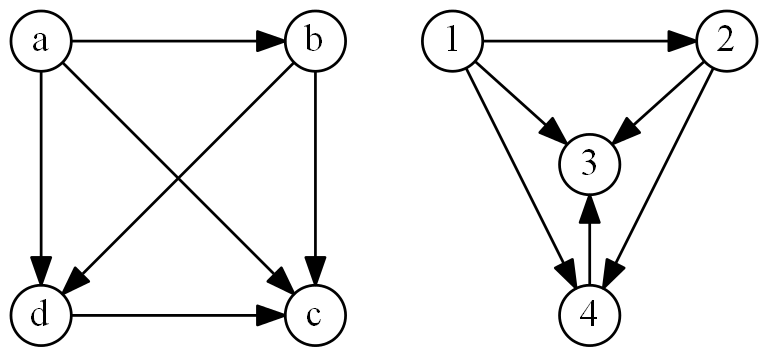
\includegraphics[width=10cm]{img/graph_izomorph.png}
	\end{center}
	\caption{Primer izomorfnih grafov z bijektivno funkcijo $f = \{(a, 1), (b, 2), (c, 3), (d, 4)\}$.}
	\label{pic_iso}
	\end{figure}


	Graf $G_p$ je izomorfen podgraf grafa $G_t$, če obstaja podgraf $G_t'$ grafa $G_t$, ki je izomorfen grafu $G_p$.
	Med grafoma $G_p$ in $G_t$ obstaja parcialen podgrafni izomorfizem, če je funkcija $f: V_p \to V_t$ injektivna in velja
	$(a,b) \in E_p \Rightarrow (f(a), f(b)) \in E_t$.
	Med grafoma $G_p$ in $G_t$ obstaja induciran podgrafni izomorfizem, če je funkcija $f: V_p \to V_t$ injektivna in velja
	$(a,b) \in E_p \Leftrightarrow (f(a), f(b)) \in E_t$. Na sliki~\ref{pic_sub_iso} vidimo, da je med $b)$ in $c)$ samo parcialni podgrafni
	izomorfizem, ker v vzorčnem grafu ni povezave $(B, C)$, medtem ko preslikavi teh vozlišč $(2, 3)$ tvorita povezavo v $c)$. Induciran 
	podgrafni izomorfizem lahko obstaja samo, če se ohranijo tudi ne-povezave.
	
	Pri reševanju problema izomorfnega podgrafa lahko ugotavljamo obstoj oz.~število podgrafnih izomorfizmov ali pa iščemo enega oz.~vse
	podgrafne izomorfizme (preslikave $f$). Najtežja je generiranje vseh preslikav - to različico rešujejo opisani algoritmi. Dodatno lahko rešujemo
	problem še na usmerjenih ali neusmerjenih ter označenih ali neoznačenih grafih.


	\begin{figure}
	\begin{center}
	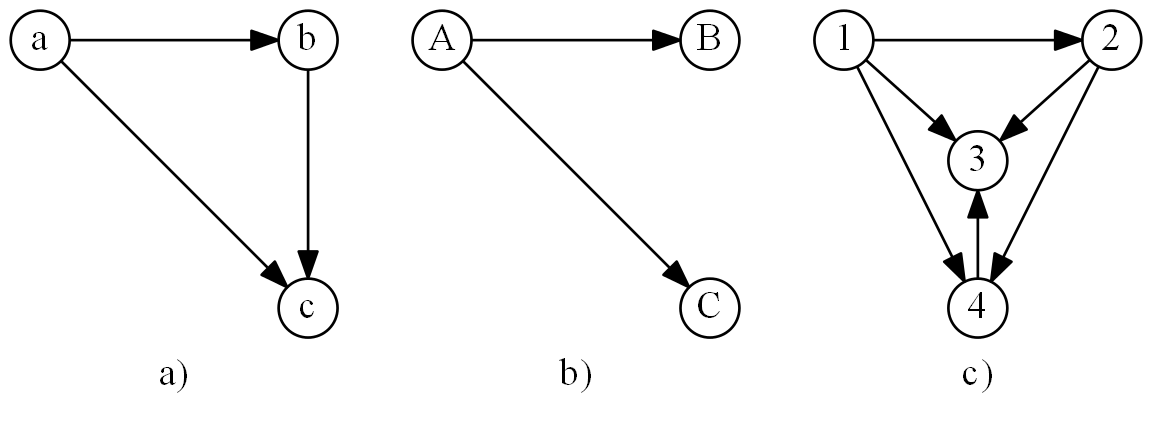
\includegraphics[width=15cm]{img/graph_sub_izomorph.png}
	\end{center}
	\caption{Med $a)$ in $c)$ obstaja induciran podgrafni izomorfizem z injektivno funkcijo $f = \{(a, 1), (b, 2), (c, 3)\}$. Med $b)$ in $c)$ obstaja
	parcialen podgrafni izomorfizem z injektivno funkcijo $f = \{(A, 1), (B, 2), (C, 3)\}$.}
	\label{pic_sub_iso}
	\end{figure}



	\section{Druge definicije}
	%rabim gamma definicije?

	Na tem mestu so zbrane pomožne definicije, ki jih uporabljamo pri opisih algoritmov za iskanje izomorfnih podgrafov.

	V neusmerjenem grafu je število povezav, ki vsebujejo vozlišče $v$, stopnja (ang.~degree) vozlišča $v$. Označimo jo z $d(v)$. Množica vozlišč
	$N(v) = \{u \in V \big| \{v, u\} \in E\}$ je množica sosedov vozlišča $v$. 
	Množica sosednjih vozlišč podgrafa $S = (V_S, E_S)$ je definirana kot 
	$N(S) = \{ n \in (V \setminus V_S) \big| \exists m \in V_S : \{n,m\} \in E \}$. 

	V usmerjenem grafu je število povezav, ki imajo vozlišče $v$ za začetek
	povezave, 	izstopna stopnja (ang.~out-degree) vozlišča. Označimo jo z $d^+(v)$.
	Število povezav, ki imajo vozlišče $v$ za konec povezave, je vstopna stopnja (ang.~in-degree) vozlišča $v$. Označimo jo z $d^-(v)$.
	Množica naslednikov
	$N^+(v) = \{u \in V \big| (v,u) \in E\}$
	so končna vozlišča povezav, ki imajo za začetek povezave vozlišče $v$.
	Množica predhodnikov 
	$N^-(v) = \{u \in V \big| (u,v) \in E\}$
	so začetna vozlišča povezav, ki imajo za konec povezave vozlišče $v$. 
	Množica izhodnih sosedov (ang.~out-neighbors) podgrafa $S = (V_S, E_S)$ je definirana kot 
	$N^+(S) = \{ n \in (V \setminus V_S) \big| \exists m \in V_S : (m,n) \in E \}$.
	Množica vhodnih sosedov (ang.~in-neighbors) podgrafa $S = (V_S, E_S)$ je definirana kot 
	$N^-(S) = \{ n \in (V \setminus V_S) \big| \exists m \in V_S : (n,m) \in E \}$.

	Rez grafa $G$ je razdelitev vozlišč $V$ v dve disjunktni množici $(A, \bar A)$. Množico povezav, kjer je en konec povezave v $A$ in drugi v
	 $\bar A$ označimo z $e(A, \bar A) = \{(u,v) \in E \big| u \in A, v \not \in A\}$. Minimalna bisekcija  grafa G je rez, ki minimizira velikost reza 
	$| e(A, \bar A) |$ po vseh množicah $A$ velikosti $\lceil | V | / 2 \rceil$.

	\TODO{\section{NP-polnost}}	


\chapter{Ullmannov algoritem}
\TODO{Intro.}


	\section{Predstavitev problema podgrafnega izomorfizma z matrikami}
	V tem algoritmu predstavimo grafe in problem reševanja podgrafnih izomorfizmov z matrikami. Matriki $P = [p_{i,j}] : 1 \le i,j \le n_p $ in
	$T = [t_{i,j}] = 1 \le i,j \le n_t$ sta matriki sosednosti grafov $G_p$ in $G_t$, kjer vrednost 1 v vrstici $i$ in stolpcu $j$ pomeni, 
	da v grafu obstaja povezava
	iz $i$ v $j$:
		\begin{equation}
		 	p_{i,j} = \left\{
			\begin{array}{l l}
			    1 & (i,j) \in E_p\\
			    0 & \text{sicer.}
			\end{array} \right.
		\end{equation}
	Matrika $M = [m_{i,j}]: 1 \le i \le n_p \wedge 1 \le j \le n_t$ predstavlja preslikavo $f: V_p \to V_t$. Vrednost 1 v v vrstici $i$ in stolpcu $j$ 
	pomeni preslikavo vozlišča
	$i \in V_p$ v $j \in V_t$:
		\begin{equation}
			m_{i,j} = \left\{
			\begin{array}{l l}
			    1 & f(i) = j\\
			    0 & \text{sicer.}
			\end{array} \right.
		\end{equation}
	Matrika $M$ je injektivna, če je v vsaki vrstici natanko ena 1 in v vsakem stolpcu največ ena 1. Samo preslikavo lahko lahko zapišemo v matrični obliki:
		\begin{equation}
			C = [c_{i,j}] = M(MT)^T
		\end{equation}
		\TODO{
		$$%\begin{equation}
			\text{mogoce tako, zaradi usmerjenih grafov? } C = [c_{i,j}] = (M(MT)^T)^T
		$$%\end{equation}
		}
	$M$ predstavlja podgrafni izomorfizem iz $G_p$ v $G_t$, če je dobljena matrika C enaka matriki sosednosti P:
		\begin{equation}
			\label{eq:ullmann1}
			c_{i,j} = p_{i,j}\;\; \forall i,j \in [1, n_p]
		\end{equation}	 
	Podana enačba velja za inducirani izomorfizem, pri enostavnem izomorfizmu je pogoj $p_{i,j} \Rightarrow c_{i, j}$.
	
	Ullmannov algoritem v osnovi generira različne matrike $M$ in jih preverja s pogojem~(\ref{eq:ullmann1}). Vseh možnih matrik $M$ je
	$\frac{n_t!}{(n_t-n_p)!}$ (ob upoštevanju pogoja za injektivnost: točno ena 1 v vrstici in največ ena 1 v stolpcu), kar je preveč za izčrpno preiskovanje.
	Algoritem zato začne z pred-procesirano matriko $M^0$~(\ref{eq:ullmann2}), na vsakem koraku pa jo še dodatno omeji~(\ref{eq:ullmann3}).
	
	
	\section{Algoritem}
	Matriko $M$ generiramo postopoma, po korakih. V danem koraku nam vrednost $m_{i,j}^k$ pove, ali se vozlišče $i \in V_p$ lahko preslika 
	v $j \in V_t$ (ima vrednost $1$) ali ne	(ima vrednost $0$). Izhajamo iz začetne matike $M^0$. V generiranju te matrike upoštevamo dejstvo, da
	se lahko vozlišče $i$ preslika v $j$ samo, če je stopnja vozlišča v vzorčnem grafu manjša ali enaka stopnji vozlišča v ciljnem grafu:
		\begin{equation}
		\label{eq:ullmann2}
		m_{i,j}^0 = \left\{ 
		  \begin{array}{l l}
		    1 & \text{$d(i) \leq d(j)$}\\
		    0 & \text{sicer.}
		  \end{array} \right.
		\end{equation}
	Pri usmerjenih grafih mora pogoj  veljati tako za vhodno kot za izhodno stopnjo.
	
	V vsakem naslednjem koraku izberemo še neobiskano vrstico. V vrstici izberemo stolpec, ki ima vrednost 1 in še ni bil izbran v nobeni prejšnji vrstici.
	Vse ostale vrednosti v vrstici postavimo na 0
	in gremo v naslednji korak. Če stolpca z vrednostjo 1 v trenutni vrstici ni, se vrnemo v prejšnji korak in izberemo drug stolpec. Ko obdelamo vse vrstice,
	se preveri pogoj~(\ref{eq:ullmann1}).
	
	Algoritem je Ullmann v izvirnem članku~\cite{ullmann} opisal s stavki GOTO, zaradi česar je težje razumljiv. Tukaj ga podajamo v bolj pregledni obliki,
	ki je popravljena in bolj podrobna različica algoritma v~\cite{zampelli-th}. Potrebujemo naslednje podatkovne strukture:
	\begin{itemize}
		\item spremenljivko $d$, ki označuje trenutno globino v preiskovalnem drevesu
		\item spremenljivko $k$, ki označuje trenutno izbrani stolpec
		\item binaren vektor $F = <F_1, \ldots, F_i, \ldots,  F_{n_p} > $, v katerem z vrednostjo 1 na $i$-tem mestu označimo, 
			da je bil stolpec $i$ že izbran, z njim zagotovimo injektivnost preslikave
		\item vektor $H = < H_1, \ldots, H_d, \ldots, H_{n_p} > $, kjer $H_d = j$ pomeni, da je na globini $d$ izbran stolpec $j$ - od tu 
			obnovimo spremenljivko $k$ pri sestopanju
		\item matriko $M$, ki predstavlja trenutno matriko združljivih parov
		\item vektor matrik $M_v = < M_1, \ldots, M_d, \ldots, M_{n_p} > $, kjer je matrika $M_d$ zadnja generirana matrika $M$ na globini $d$ - od
			tu obnovimo matriko $M$ pri sestopanju
	\end{itemize}

	Prevdokoda algoritma je podana v \refalg{alg:ullmann1}. V vrsticah 1--2 inicializiramo vse spremenljivke -- začnemo z začetno matriko $M^0$, 
	na globini 1 in brez izbranega stolpca. V vrstici 3 shranimo matriko $M$ za prvi korak - matriko vedno shranjujemo pred vstopom v naslednji korak. 	
	Zanka v vrstici 4 še izteče, ko sestopimo iz obdelave prve vrstice, torej ko v prvi vrstici zmanjka neobiskanih stolpcev. V vrstici 5 poskrbimo, da 
	algoritem sestopi, če ne najdemo ustreznega stolpca. V vrstici 6 preverimo, če v trenutni vrstici obstaja še neobiskan stolpec. Ta stolpec mora biti še
	neizbran v trenutni vrstici ($j > k$), biti združljiv s trenutno vrstico ($m_{d,j} = 1$) in ne sme biti izbran v	katerem od prejšnjih korakov ($F_j=0$;
	pogoj za injektivno preslikavo). Sama izbira stolpca poteka v vrsticah 8--10, ko vrednost $k$ postavimo na izbrani stolpec, v vrstici 7 pa preprečimo 
	sestopanje, saj bomo v naslednji ponovitve zanke ali povečali globino ali pa ostali na isti globini.
	V vrstici 11 postavimo vse neizbrane stolpce v vrstici na $0$, torej izbrani stolpec označimo tudi v matriki $M$. Pogoj v vrstici 12 zaenkrat ignorirajmo.
	Če nismo prišli do dna preiskovalnega
	drevesa (vrstica 13), gremo v naslednji korak (vrstica 14): shranimo zadnji izbrani stolpec na trenutni globini ($H_d \gets k$), stolpec označimo kot
	že izbranega ($F_k \gets 1$), povečamo globino ($d \gets d + 1$), resetiramo izbiro stolpca za naslednji korak ($k \gets 0$) in shranimo matriko $M$
	za naslednji korak ($M_d \gets M$; od tukaj bomo obnavljali matriko $M$ ob vračanju v tisti korak).
	Če smo obdelali že vse vrstice v matriki $M$, potem v vrstici 16 preverimo, če matrika ustreza pogoju~(\ref{eq:ullmann1}), torej če matrika predstavlja
	podgrafni izomorfizem. Če pogoj drži, jo ustrezno shranimo ali izpišemo. V vrstici 18 obnovimo matriko $M$. Tako bomo
	v naslednji ponovitvi zanke preverili, če je v zadnji vrstici še kakšen primeren stolpec. Vrstici 19 in 20, tako kot vrstico 12, zaenkrat preskočimo.
	Vrstice 21--24 skrbijo za sestopanje, ki se izvede, če v trenutni 
	vrstici ni nobenega primernega stolpca več. V vrstici 22 sprostimo zadnji izbrani stolpec ($F_k \gets 0$) in znižamo globino. Nato v vrstici 24 obnovimo
	matriko $M$ in v $k$ obnovimo nazadnje izbrani stolpec na tej globini.
	
\begin{algorithm}
\caption{Ullmannov algoritem}
\label{alg:ullmann1}
\begin{algorithmic}[1]
	\Require Matriki sosednosti $P$ in $T$, začetna matrika $M^0$
	\Ensure Vse $n_p \times n_t$ matrike $M$, ki predstavljajo preslikave podgrafnih izomorfizmov				
	\State $M \gets M^0; d \gets 1; H_1 \gets 0; k \gets 0; backtract \gets true$								
	\For{$i $ in$ [1, n_p]$} $F_i \gets 0;$ \EndFor													
	\State $M_1 \gets M^0$																	
	\While{$d \not = 0$}																		
		\State $backtrack \gets true$													
		\If{$(\exists j : j > k \wedge m_{d,j} = 1 \wedge F_j = 0)$}			
			\State $backtrack \gets false$
			\Repeat 
				\State $k \gets k +1$ 															
			\Until{$m_{d,k} = 1 \vee F_k = 1$}													
			\State $\forall j \not = k : m_{d,j} \gets 0$										\label{alg:ullmann1.11}
			\If {$[\;refine(M, P, T)\;]$}
				\If {$d < n_p$}																	
					\State $H_d \gets k; F_k \gets 1; d \gets d+1; k \gets 0; M_d \gets M$
				\Else																			
					\If {$<$ condition(\ref{eq:ullmann1}) $>$}											
						\State $<$ store $M$ $>$
					\EndIf													
					%\If{$\exists j : j > k \wedge m_{d,j} = 1 \wedge F_j = 0$}								
						\State $M \gets M_d$		
					%\EndIf
				\EndIf
			\Else
				\State $M \gets M_d$
			\EndIf
		\EndIf
		
		\If{$backtract$}																		
			\State $F_k \gets 0; d \gets d-1;$													
			\If{$d > 0 $}																	
				\State $M \gets M_d; k \gets H_d;$												
			\EndIf
		\EndIf
	\EndWhile
\end{algorithmic}
\end{algorithm}

	Velik del podanega algoritma se ukvarja s sestopanjem in obnavljanjem stanja pri sestopanju. Zato v \refalg{alg:ullmann3} podajamo še rekurzivno 
	različico algoritma. V tej različici za sestopanje in obnavljanje stanja skrbi sama rekurzija in je potek algoritma bolj očiten. V vrsticah 1 in 2 je
	inicializacija, le da sedaj potrebujemo manj spremenljivk. V vrstici 3 začnemo preiskovanje na globini 1. V vrstici 7 shranimo trenutno matriko $M$,
	ki jo bomo obnavljali ob sestopanju (ponovno zaenkrat ignoriramo del v oglatih oklepajih). V vrstici 8 je zanka, ki preveri vse stolpce. Ko pridemo do
	ustreznega (vrstica 9), vse ostale stolpce postavimo na 0 (vrstica 10), in označimo stolpec kot izbran (vrstica 11). Če smo v zadnji vrstici matrike $M$,
	potem preverimo pogoj~\ref{eq:ullmann1} in če smo našli izomorfizem, shranimo trenutno matriko $M$ (vrstice 12-14). Če to ni zadnja vrstica, gremo
	v naslednji korak (vrstica 16). Ob sestopanju obnovimo matriko $M$ in označimo trenutni stolpec kot neizbran (vrstica 17).

\begin{algorithm}
\caption{Ullmannov algoritem - rekurzivna različica}
\label{alg:ullmann3}
\begin{algorithmic}[1]
	\Require Matriki sosednosti $P$ in $T$, začetna matrika $M^0$
	\Ensure Vse $n_p \times n_t$ matrike $M$, ki predstavljajo preslikave podgrafnih izomorfizmov				
	\State $M \gets M^0$
	\For{$i $ in$ [1, n_p]$} $F_i \gets 0;$ \EndFor
	\State $step(1)$
	\Statex
	\Function{step}{d}
		\If{$[! \; refine(M, P, T)\; ]$}
			\State \Return
		\EndIf
		\State $M_d \gets M$
		\ForAll{$k \in [1,n_t]$}
			\If{$m_{d,k} = 1 \wedge F_k = 0$}
				\State $\forall j \not = k : m_{d,j} \gets 0$
				\State $F_k \gets 1$
				\If{$d = n_p$}
					\If {$<$ condition(\ref{eq:ullmann1}) $>$}
						\State $<$ store $M$ $>$
					\EndIf
				\Else
					\State $step(d+1)$
				\EndIf
				\State $F_k \gets 0; M \gets M_d$
			\EndIf
		\EndFor
	\EndFunction
\end{algorithmic}
\end{algorithm}


	\section{Omejevanje prostora preiskovanja}
	Ullmann je opazil, da lahko z dodatnim procesiranjem matrike $M$ na vsakem koraku dodatno omejimo prostor preiskovanja, torej da več 1 postavimo
	na 0. Če se bo vozlišče $i$ v preslikalo v vozlišče $j$, potem se mora tudi vsako sosednje vozlišče vozlišča $i$ preslikati v eno od 
	sosednjih vozlišč vozlišča $j$. Za vsak $m_{i,j} = 1$ preverimo pogoj:
	\begin{eqnarray}
	\label{eq:ullmann3}
	\nonumber 
	\forall x \in N_{p}(i) & \Rightarrow & \exists y \in N_t(j) \wedge m_{x,y} = 1
	\\
	\forall x \in [1, n_p] : p_{i,x} = 1 & \Rightarrow & \exists y \in [1, n_t] : t_{j,y} = 1 \wedge m_{x,y} = 1
	\end{eqnarray}
	Če pogoj ni izpolnjen, postavimo vrednost $m_{i,j}$ na 0. Vsaka sprememba v matriki lahko vpliva na pogoj pri ostalih vozliščih, zato postopek
	ponavljamo, dokler pri pregledu celotne matrike ne naredimo nobene spremembe. Ta pogoj je hkrati tudi zadosten za preverjanje podgrafnega 
	izomorfizma, zato lahko v algoritmih z njim nadomestimo pogoj~(\ref{eq:ullmann1}).
	
	Psevdokoda postopka je podana v~\refalg{alg:ullmann2}. Za vsak
	združljiv par (vrstica 4) preverimo pogoj~(\ref{eq:ullmann3}) v vrstici 5. Če pogoj ni izpolnjen, označimo par kot nezdružljiv (vrstica 6). Poleg tega
	označimo, da bo celoten postopek potrebno ponoviti ($fixpoint \gets false$). Ob spremembi v matriki $M$ preverimo še, če trenutna vrstica sedaj vsebuje
	same 1 (vrstica 7). V tem primeru namreč izomorfizem ni več mogoč, zato vrnemo $false$ (vrstica 8). 

	Podani algoritem je v \refalg{alg:ullmann1} in \refalg{alg:ullmann3} že vključen, klic funkcije $refine$ je v oglatih oklepajih, ki smo jih predhodno
	ignorirali.

%\begin{spacing}{1} 
\begin{algorithm}
\caption{Dodatno omejevanje prostora}
\label{alg:ullmann2}
\begin{algorithmic}[1]
	\Require Matrika $M$ in sosednostni matriki $P$ in $T$
	\Ensure $true$ če je bila M omejena, $false$ če kakšna vrstica ne vsebuje nobene 1
	\Function{refine}{$M$, $P$, $T$}
		\Repeat
			\State $fixpoint \gets true$
			\For{$\forall (i,j): m_{i,j} = 1$}
				\If{condition (\ref{eq:ullmann3}) is not satisfied}
					\State $m_{i,j} \gets 0; fixpoint \gets false;$
					\If{$\forall k : m_{i,k} = 0$}
						\State \Return false
					\EndIf
				\EndIf
			\EndFor
		\Until{$fixpoint$}
		\State \Return $true$
	\EndFunction
\end{algorithmic}
\end{algorithm}
%\end{spacing}

	Prostorska zahtevnost celotnega algoritma je $O(n_p^2 n_t)$. Na vsaki globini shranimo matriko $M$, ki je velikosti $n_p n_t$, maksimalna globina pa 
	je $n_p$. Časovna kompleksnost funkcije $refine$ je $O(n_p n_t d_{max})$, kjer je $d_{max}$ največja možna stopnja vozlišča. Pogoj preverjamo za
	vsak	element matrike $M$, časovna zahtevnost pogoja pa je $d_{max}$, ker preverjamo samo sosede. Postopek preverjanja se sicer ponavlja do fiksne
	točke, ampak vsaka ponovitev dodatno poreže preiskovalno drevo, zato je ena ponovitev najslabši primer. Celoten algoritem ima časovno zahtevnost
	$O(n_p! n_p n_t d_{max})$. V posamezni ponovitvi zanke je funkcija $refine$ najzahtevnejša, število ponovitev pa je reda $n_p!$.


	\section{Izboljšave}
	\TODO{Ref.}
	
	V \refalg{alg:ullmann1} obiskujemo vozlišča iz vzorčnega grafa po vrsti, glede na sam zapis grafa z matriko. Drugačen vrsti red obiskovanja lahko
	pohitri algoritem, če čim hitreje ustavi preiskovanje poddreves, ki nimajo rešitve. Nekaj možnih hevristik:
	\begin{itemize}
	\item Najprej vozlišča z večjo stopnjo -- taka vozlišča imajo običajno manj kandidatov za preslikavo.
	\item Preiskovanje v širino, znotraj iste globine pa po stopnji
	\item Najboljši najprej -- začnemo z vozliščem z največjo stopnjo, v vsakem naslednjem koraku pa med sosedi že obiskanih vozlišč izberemo vozlišče z
	največjo stopnjo.
	\end{itemize}
	
	Omejevanje prostora iskanja s funkcijo $refine$ izkorišča dejstvo, da mora za vsakega soseda vozlišča $i$ obstajati združljiv sosed vozlišča $j$.
	Podobno pa velja, če še $i$ preslika v $j$, potem sosedje vozlišča $i$ ne morejo biti združljivi z vozlišči, ki niso sosedje vozlišča $j$:
	\begin{eqnarray}
	\label{eq:ullmann_imp1}
	\forall x \in N_p(i) \;\; \forall y \not \in N_t(j) : m_{x,y} = 0
	\end{eqnarray}
	Pri iskanju induciranega podgrafnega izomorfizma pa tudi v nasprotno smer:
	\begin{eqnarray}
	\label{eq:ullmann_imp2}
	\forall y \in N_t(j) \;\; \forall x \not \in N_p(i) : m_{x,y} = 0
	\end{eqnarray}
	Ta postopek lahko za razliko od $refine$ uporabimo samo za tiste $(i, j)$, za katere vemo, da bo $m_{i,j}$ obdržala vrednost 1. V \refalg{alg:ullmann1}
	bi ga uporabili v vrstici \ref{alg:ullmann1.11} nad $m_{d,k}$. Postopek zmanjša prostor preiskovanja za sosednja vozlišča, kar lahko dobro izkoristita 
	zadnji dve hevristiki iz prejšnjega odstavka. Pri njiju bodo namreč sosednja vozlišča hitro na vrsti za preiskovanje.
	
	Izboljšati je mogoče tudi prostorsko zahtevnost. Osnovni algoritem namreč na vsakem koraku shrani celotno matriko $M$. Namesto sklada matrik lahko
	uporabimo persistentno matriko. Ob spremembi vrednosti v matriki iz 1 v 0 na sklad shranimo koordinate spremembe. Ob sestopanju iz sklada
	preberemo koordinate sprememb in na ustreznih mestih vrednost povrnemo nazaj v 1. Ker je sprememb kvečjemu $n_p n_t$, se prostorska
	zahtevnost zmanjša na $O(n_p n_t)$.
	


\chapter{VF2}

\chapter{Subsee}

\chapter{Eksperimentalna primerjava algoritmov}
	\section{}

\chapter{Sklepne ugotovitve}


\begin{thebibliography}{99}

	%@article{LipetsVG09,
	%  title = {Subsea: an efficient heuristic algorithm for subgraph isomorphism},
	%  author = {Vladimir Lipets and Natalia Vanetik and Ehud Gudes},
	%  year = {2009},
	%  doi = {http://dx.doi.org/10.1007/s10618-009-0132-7},
	%  researchr = {http://researchr.org/publication/LipetsVG09},
	%  cites = {0},
	%  citedby = {0},
	%  journal = {Data Min. Knowl. Discov.},
	%  volume = {19}, %številka?
	%  number = {3}, % zvezek?
	%  pages = {320-350},
	%}
	\bibitem{subsea} V.~Lipets, N.~Vanetik, E.~Gudes, ``Subsea: an efficient heuristic aglorithm for subgraph isomorphism",
		\textit {Data Mining and Knowledge Discovery}, št.~19, zv.~3, 2009, str.~320--350.

	% Journal of the ACM, Vol. 23, No. 1. (January 1976), pp. 31-42
	\bibitem{ullmann} J.~R.~Ullmann, ``An Algorithm for Subgraph Isomorphism",
		\textit{Journal of the ACM}, št.~23, zv.~1, str.~31-42, 1976

	\bibitem{zampelli-th} S. Zamplelli, ``A constraint programming approcah to subgraph isomorphism", Doktorska disertacija, 
	Universit\'{e} catholique de Louvain, D\'{e}partement d’Ing\'{e}nierie Informatique, Belgija, 2008.

\end{thebibliography}
\end{document}

